% Chapter Template

\chapter{Kociemba Bug} % Main chapter title

\label{sec:Kociemba} % Change X to a consecutive number; for referencing this chapter elsewhere, use \ref{ChapterX}


Let me discuss in this appendix in more details the issue I mentioned in section \ref{sec:ResRubiks333} regarding the \textit{poor} interface of the kociemba (3x3x3) library.
\\
\\
I personally like to follow the great Scott Meyers' advice (see item 18 of \cite{meyers2005effective}), which is to not merely make interfaces easy to use, but also difficult to misuse. In that instance, I would argue they have made it very easy to shoot oneself in the foot with their interface which assumes the cubes passed to the solver are in \textit{standard} form (my terminology), not only without making that explicit anywhere, but worse than that: sometimes non standard initial configuration raise an exception, sometimes not and returning a solution which is not really one! So what is the problem exactly?
\\
\\
To start with, let us remember from chapter \ref{sec:Puzzles} that each \textbf{RC} configuration has 24 equivalent configurations under invariance by full rotation of the cube in space. Out of 24 equivalent configurations, and for an observer facing the cube, there is only one whose center front (F) cubie is red and center up (U) cubie is white.
\\
\\
In hkociemba (the third parties 2x2x2 implementation which I used under the hood of my KociembaSolver), the problem of these equivalent puzzles is irrelevant (since full cube rotation can always be achieved by 2 rotations of 2 opposite faces in opposite directions, e.g. FB' is equivalent to full cube rotation around F (CF in my jargon)). That being said, the hkociemba is smarter than just using the equivalence between full cube rotation and two faces' rotations. It does automatic color scheme recognition when passed a \textit{cube string}, and gets a smart solution given that coloring scheme. For instance, if we pass it a solved configuration, but not in standard form, it knows there is no need to do anything. In the general case of a scrambled cube, it will also endeavour to find solutions to the closest among the 24 equivalent solved configurations. Let's look at the following concerete example:


\afblue
\paragraph{}{\textbf{Kociemba bug -- 2x2x2 \textbf{RC} -- example of good interface design}}
\begin{python}
#####################################################################
from rubiks.puzzle.puzzle import Puzzle
from rubiks.solvers.solver import Solver
from rubiks.solvers.kociembasolver import KociembaSolver
from_kociemba = KociembaSolver.from_kociemba
to_kociemba = KociembaSolver.to_kociemba
#####################################################################
puzzle_type = Puzzle.rubiks_cube
n=2
init_from_random_goal=False
cube = Puzzle.factory(**globals()).get_equivalent()[-1].apply_random_moves(nb_moves=1)
solver_type = Solver.kociemba
solver = Solver.factory(**globals())
print(solver.solve(cube))
#####################################################################
\end{python}
\black

which, subject to randomness, gave me the following scrambled cube and solution:

\begin{figure}[H]
\centering
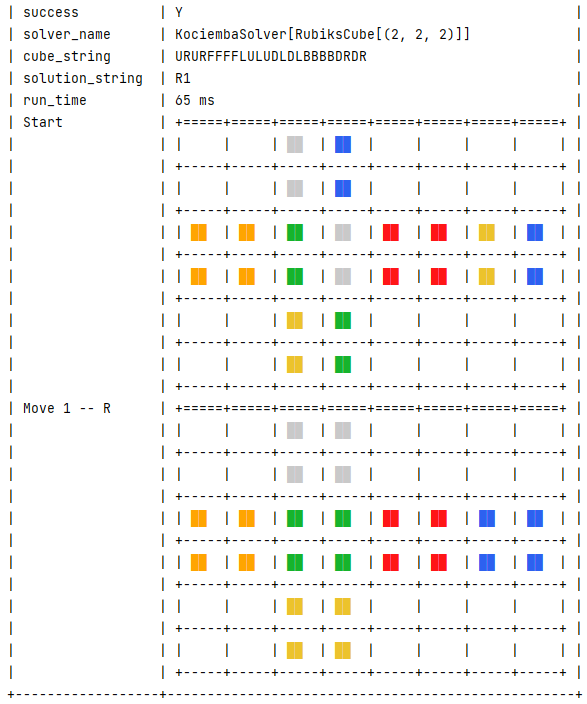
\includegraphics[scale=0.6]{./Figures/KociembaBug222}
%\decoRule
\caption[Kociemba Bug]{2x2x2 \textbf{RC} -- hkociemba finds path to closest of the 24 equivalent goals}
\label{fig:KociembaBug222}
\end{figure}
As we can see, hkociemba happily returned a 1-move solution R to green F, white U, instead of the costlier solution it would have taken to get to \textit{standard} form red F white U (clearly at a cost of 3 with solution RUD').
\\
\\
In the 3x3x3 case, things are not quite that simple. There is no way to reproduce full cube rotation from faces rotations alone, since the center cubies will never move via the latter, but do via the former. If we run the equivalent of the above problem with the (3x3x3) kociemba library, we silently get to a false solution as is apparent from printing the resulting cube.
\afblue
\paragraph{}{\textbf{Kociemba bug -- 3x3x3 \textbf{RC} -- example of \textbf{bad} interface design}}
\begin{python}
#####################################################################
from kociemba import solve
#####################################################################
from rubiks.puzzle.puzzle import Puzzle
from rubiks.solvers.kociembasolver import KociembaSolver
from_kociemba = KociembaSolver.from_kociemba
to_kociemba = KociembaSolver.to_kociemba
#####################################################################
puzzle_type = Puzzle.rubiks_cube
n=3
init_from_random_goal=False
cube = Puzzle.factory(**globals()).get_equivalent()[-1].apply_random_moves(nb_moves=1)
print(cube)
cube_string = to_kociemba(cube)
solution = solve(cube_string)
print('Kociemba Solution:', solution)
print(cube.apply_moves(from_kociemba(solution)))
###################################################################
\end{python}
\black

\begin{figure}[H]
\centering
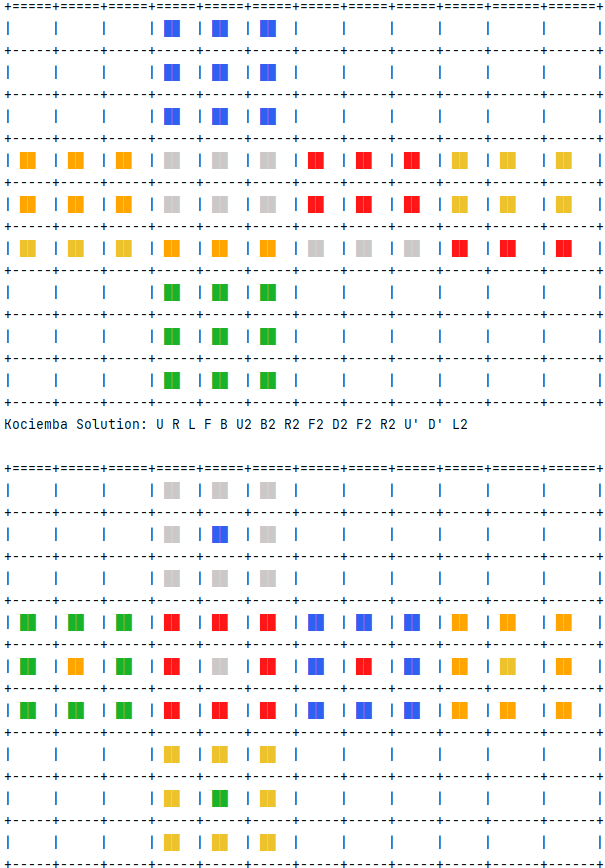
\includegraphics[scale=0.6]{./Figures/KociembaBug333}
%\decoRule
\caption[Kociemba Bug]{3x3x3 \textbf{RC} -- kociemba does not check center cubies and returns wrong solution}
\label{fig:KociembaBug333}
\end{figure}
In order to counteract that, and make the comparisons between Kociemba 3x3x3 and other solvers and methods fairer, I have had to implement a layer on top of kociemba. My Kociemba solver basically will check if a cube is in \textit{standard} form, and if not, it will find the sequence of full cube rotations that bring us to an equivalent configuration in \textit{standard} form, pass that to equivalent \textit{standard} cube to kociemba, and stich the cube rotation to the kociemba solution (treating cube rotation as 0 cost everywhere in the code). That way, we seamlessly get to an answer that makes sense from kociemba, without the user having to worry about whether or not the cube they are passing as input is in \textit{standard} form or not! Running the same example as above via my KociembaSolver, we get the expected result, composed of 3 cube rotations to bring it to \textit{standard} form, followed by one face rotation to solve it:

\afblue
\paragraph{}{\textbf{Kociemba bug -- 3x3x3 \textbf{RC} --  massage to fix the broken interface}}
\begin{python}
#####################################################################
from rubiks.puzzle.puzzle import Puzzle
from rubiks.solvers.solver import Solver
from rubiks.solvers.kociembasolver import KociembaSolver
from_kociemba = KociembaSolver.from_kociemba
to_kociemba = KociembaSolver.to_kociemba
#####################################################################
puzzle_type = Puzzle.rubiks_cube
n=3
init_from_random_goal=False
cube = Puzzle.factory(**globals()).get_equivalent()[-1].apply_random_moves(nb_moves=1)
solver_type = Solver.kociemba
solver = Solver.factory(**globals())
print(solver.solve(cube))
###################################################################
\end{python}
\black

\begin{figure}[H]
\centering
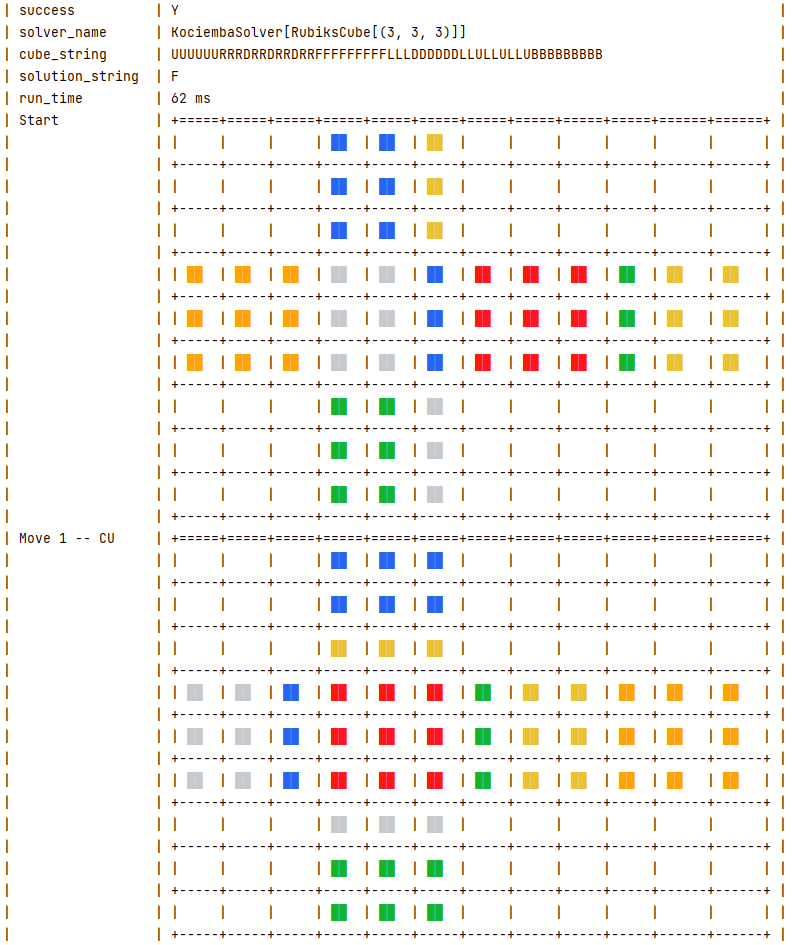
\includegraphics[scale=0.5]{./Figures/KociembaBug333Fix1}
%\decoRule
\label{fig:KociembaBug333Fix1}
\end{figure}

\begin{figure}[H]
\centering
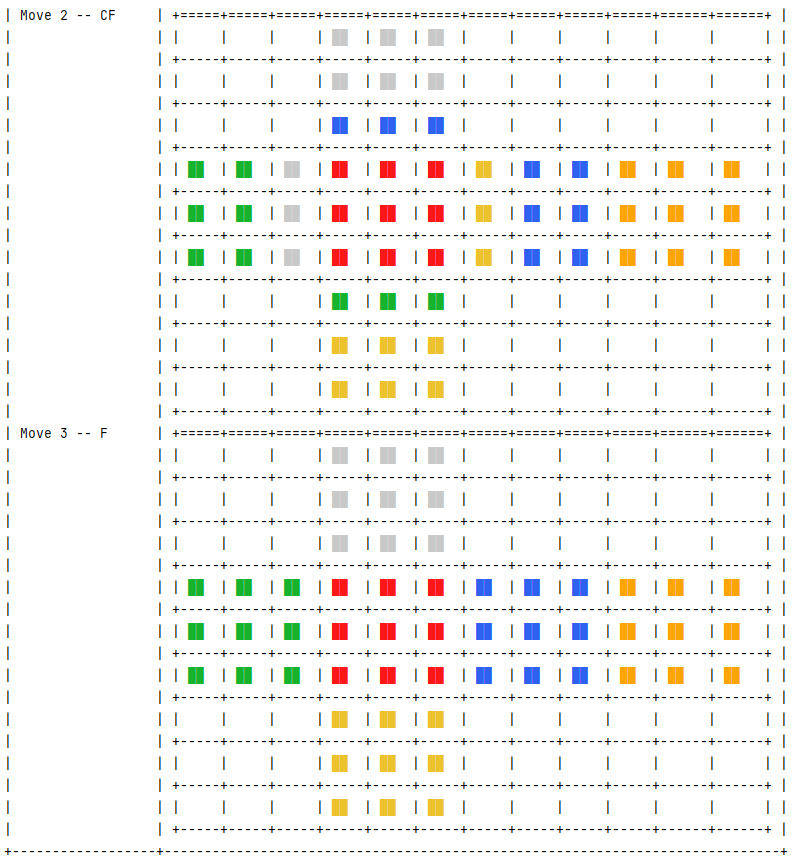
\includegraphics[scale=0.5]{./Figures/KociembaBug333Fix2}
%\decoRule
\caption[Kociemba Bug Fix]{3x3x3 \textbf{RC} -- Fixed kociemba interface}
\label{fig:KociembaBug333Fix2}
\end{figure}







%-----------------------------------
%	SECTION 1
%-----------------------------------




